\setcounter{section}{0}   %sita automatiskai atnaujina \appendix komanda
\renewcommand*{\thesection}{S.\arabic{section}}
\renewcommand{\thechapter}{S}
\renewcommand{\thefigure}{S.\arabic{figure}}   %raide S ihardcodinta. Galima svelniau pvz su komanda \thechapter
\setcounter{figure}{0}
\renewcommand{\theequation}{S.\arabic{equation}}
\setcounter{equation}{0}
\renewcommand{\thetable}{S.\arabic{table}}
\setcounter{table}{0}
%jeigu yra dar ko nors, pvz algoritmu, teor ir pan, irgi reikia atnaujinti

\phantomsection
\addcontentsline{toc}{chapter}{Santrauka (Summary in Lithuanian)}

	
% \parammarks{Santrauka (Summary in Lithuanian)}

\chapter*{Santrauka (Summary in Lithuanian)}
\label{cha:summary_lt}

\lithuanian   %nustatome lietuviu kalba
\sisetup{output-decimal-marker = {,}}  %lietuviski kableliai ir pan
\sisetup{exponent-product=\ensuremath{\cdot}}

% !TEX encoding = UTF-8 Unicode

\pagestyle{plain}

%\lithuanian

\phantomsection % Removes warning form hyperref package
\section*{Tyrimų sritis}
\addcontentsline{toc}{section}{Research Area / Tyrimų sritis}

Pasitelkus kompiuterinį modeliavimą disertacijoje tiriamos su\-dė\-tin\-gos cheminės ir biofizikinės sistemos, kurios yra aprašomos dalinių išvestinių lygtimis (DIL) su netiesinėmis kraštinėmis sąlygomis ir DIL sudėtingos geometrijos (nestačiakampėse) srityse. Šios DIL sprendžiamos baigtinių skirtumų metodu ir kitais skaitiniais algoritmais. 

%Disertacijoje tiriamos sudėtingos cheminės ir biofizikinės sistemos naudojant kompiuterinį modeliavimą. Šios sistemos yra aprašomos dalinių išvestinių lygtimis (DIL) su netiesinėmis kraštinėmis sąlygomis ir DIL sudėtingos geometrijos (nestačiakampėse) srityse. Šios DIL sprendžiamos baigtinių skirtumų metodu ir kitais skaitiniais algoritmais.  
%The study is focused on computer modelling of complex chemical and biophysical systems, which are described by partial differential equations (PDEs) with nonlinear boundary conditions and PDEs in various complex (non-rectangular) domains. Differential problems are solved using numerical methods
%Tyrimas skirtas išspręsti dalinių išvestinių lygtims (DIL) su netiesinėmis kraštinėmis sąlygomis sistemas ir išspręsti DIL sudėtingos geometrijos (nestačiakampėse) srityse, naudojant skaitinius metodus.

DIL sprendimo su netiesinėmis kraštinėmis sąlygomis problemos kyla dėl cheminių ir biologinių procesų matematinio modeliavimo. 
Tyrimai nestačiakampėse srityse yra aktualūs dėl poreikio įvertinti matavimo prietaisų paklaidas, atsirandančias dėl geometrijos nukrypimo nuo standarto.
%Tyrimai nestačiakampėse srityse yra aktualūs dėl poreikio modeliuoti nukrypimus nuo normos įrangoje, naudojamoje cheminiams ir biologiniams eksperimentams. 
DIL netiesinės sistemos yra pritaikytos tyrinėti chemoterapinių vaistų patekimą į audinius.





\section*{Tikslas}
\addcontentsline{toc}{section}{Tikslas} 
...





%--------------- SECM Redox reakciju skyrius ---------------------------------
%--------------------------------------------------------------------------

\section{SECM modeliavimas oksidacijos-redukcijos konkurencijos režime}
\label{sec:santr_reakc}



\subsection{Matematinis modelis}

Dėl simetrijos aplink centrinę elektrodo ašį modelis užrašomas cilindrinėse koordinatėse. Cilindro formos srityje atliekami SECM matavimai yra pakeisti į 2D sritį \ref{fig:santr_Domain} pav.


\begin{figure}[ht!]
\centering
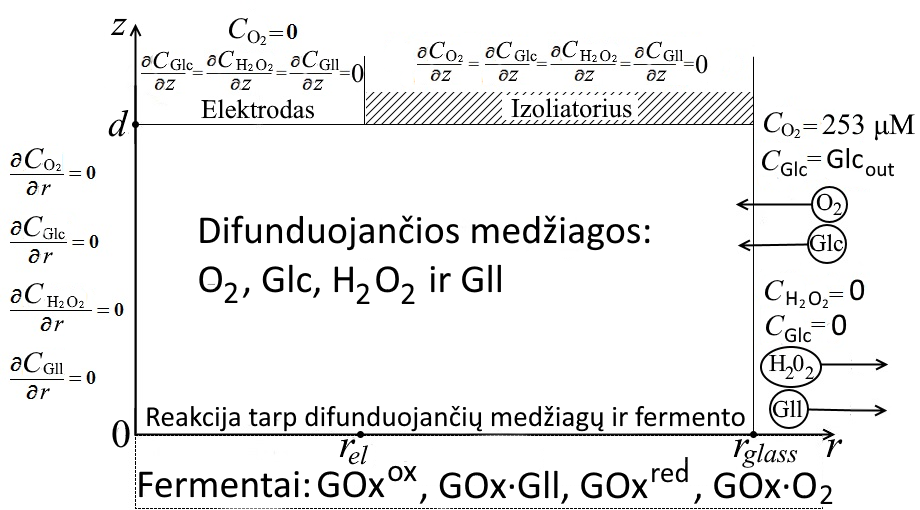
\includegraphics[width=0.8\linewidth]{summary/Model_domainLT.png}
\caption{Modeliavimo srities schema. Pavaizduotos $8$ modeliuotos medžiagos - $4$ difunduojantys reagentai bei $4$ fermento GOx formos, kraštinės sąlygos 4-ioms difunduojančioms medžiagoms ir išorinis srautas.}
\label{fig:santr_Domain}
\end{figure}

Difuzijos procesai išreiškiami antruoju Fiko dėsniu:
\begin{equation}
  \begin{aligned}\label{eq:santr_eq1}
  \frac{\partial C_{O_2}}{\partial t} &= D_{O_2}\,\Delta C_{O_2},\\
  \frac{\partial C_{Glc}}{\partial t} &= D_{Glc}\,\Delta C_{Glc},\\
  \frac{\partial C_{H_2 O_2}}{\partial t} &= D_{H_2 O_2} \,\Delta C_{H_2 O_2},\\
  \frac{\partial C_{Gll}}{\partial t} &= D_{Gll}\,\Delta C_{Gll},  \quad 0<t\leq T,\; 0<z<d,\; 0<r<r_{glass}.
  \end{aligned}
\end{equation}
Šiose lygtyse:
\begin{itemize}
  \item[] $C_{O_2}$, $C_{Glc}$, $C_{H_2 O_2}$ ir $C_{Gll}$ yra atitinkamų difunduojančių re\-a\-gen\-tų koncentracijos, kurios išreiškiamos kaip laiko $t$, er\-dvi\-nių ko\-or\-di\-na\-čių $z$ ir $r$ funkcijos. 
  \item[] $D_{O_2}$, $D_{Glc}$, $D_{H_2 O_2}$ ir $D_{Gll}$ yra difuzijos koeficientai.
  \item[] $d$ yra atstumas tarp fermentu modifikuoto paviršiaus ir elektrodo. Skaitinio eksperimento metu $d$ keičiamas nuo $\SI{1}{\um}$ iki $\SI{120}{\um}$. Tai atitinka elektrodo stumdymą aukštyn ir žemyn cheminio eksperimento metu.
  \item[] $r_{glass} = \SI{80}{\um}$ yra izoliuotos srities spindulys.
  \item[] $T$ yra skaičiavimo eksperimento trukmė, matuojama sekundėmis.
  \item[] Laplaso operatorius $\Delta$ cilindrinėse koordinatėse su centrine simetrija yra
  \begin{equation*}
  \Delta C = \frac{1}{r}\frac{\partial C }{\partial r} \left( r\frac{\partial C }{\partial r} \right) + \frac{\partial^{2} C}{\partial z^{2}}.
  \end{equation*}
\end{itemize}




\british  %griztame prie anglu kalbos